
\documentclass[preprint,12pt]{elsarticle}

\usepackage[spanish]{babel}
\usepackage{amssymb}
\usepackage{graphicx}
\usepackage{lineno}
\usepackage[utf8]{inputenc}
\usepackage{url}
\usepackage{natbib} 
\usepackage{amsmath} 
\usepackage{amssymb} 
\usepackage{float}

\begin{document}
	
	\begin{frontmatter} 

		\title{\huge Informe de Laboratorio 09 - Instalación y Gestión de una base de datos MongoDB}
		
		\author{Pedro Luis, Mamani Mamani         	(2010038808)} 
		\address{Escuela Profesional de Ingeniería de Sistemas}
		\address{Universidad Privada de Tacna}
		\address{Tacna, Perú}
	\end{frontmatter}



\section{INFORMACIÓN GENERAL} 

\subsection {\textbf{Objetivos}}
\begin{itemize}
	\item Instalación de mongodb
	\item Usar comandos basicos en mongodb
\end{itemize}

\subsection {\textbf{REQUERIMIENTOS}}
\begin{itemize}
	\item Conocimientos
Para el desarrollo de esta práctica se requerirá de los siguientes conocimientos básicos: Conocimientos básicos de administración de base de datos MongoDB, Conocimientos básicos de formato JSON.
\end{itemize}


\section{Marco Teórico}


\subsection {\textbf{Mongodb}}
MongoDB es un sistema de base de datos NoSQL orientado a documentos de código abierto. En lugar de guardar los datos en tablas, tal y como se hace en las bases de datos relacionales
\subsection {\textbf{JSON}}
JSON es un formato de texto sencillo para el intercambio de datos. Se trata de un subconjunto de la notación literal de objetos de JavaScript, aunque, debido a su amplia adopción como alternativa a XML, se considera un formato independiente del lenguaje.


\section{PROCEDIMIENTO}

\subsubsection{\textbf{Paso 1: Crear las carpeta de almacenamiento y configuracion de MongoDB.}}
\begin{figure}[H]
	\begin{center}
		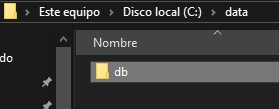
\includegraphics[width=12cm]{./IMAGENES/1} 
	\end{center}
\end{figure}
\begin{figure}[H]
	\begin{center}
		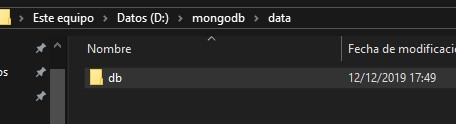
\includegraphics[width=12cm]{./IMAGENES/2} 
	\end{center}
\end{figure}

\subsubsection{\textbf{Iniciar el servidor del servicio de MongoDB: mongod.}}

\begin{figure}[H]
	\begin{center}
		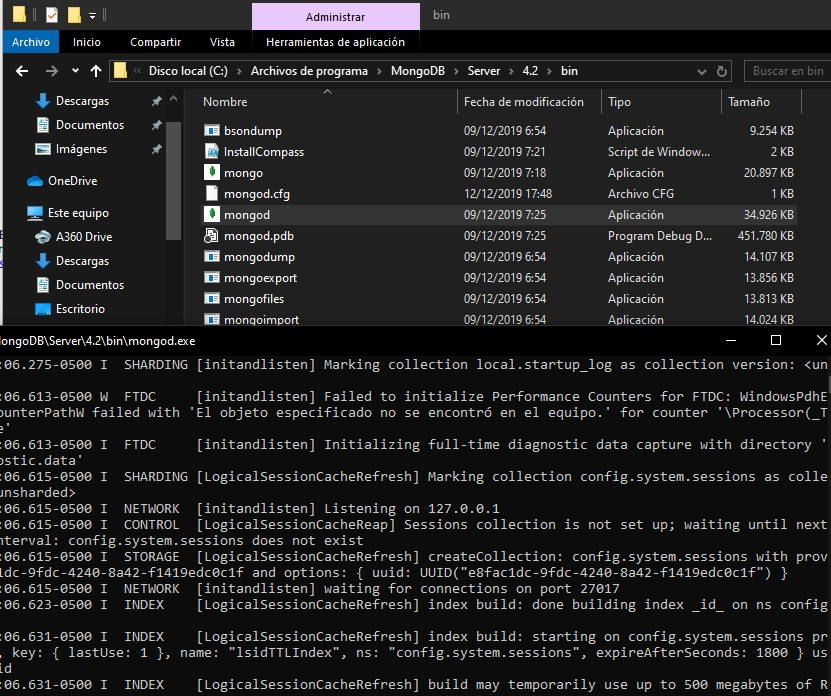
\includegraphics[width=12cm]{./IMAGENES/3} 
	\end{center}
\end{figure}

\subsubsection{\textbf{Importar un archivo JSON por medio de studio 3T}}
\begin{figure}[H]
	\begin{center}
		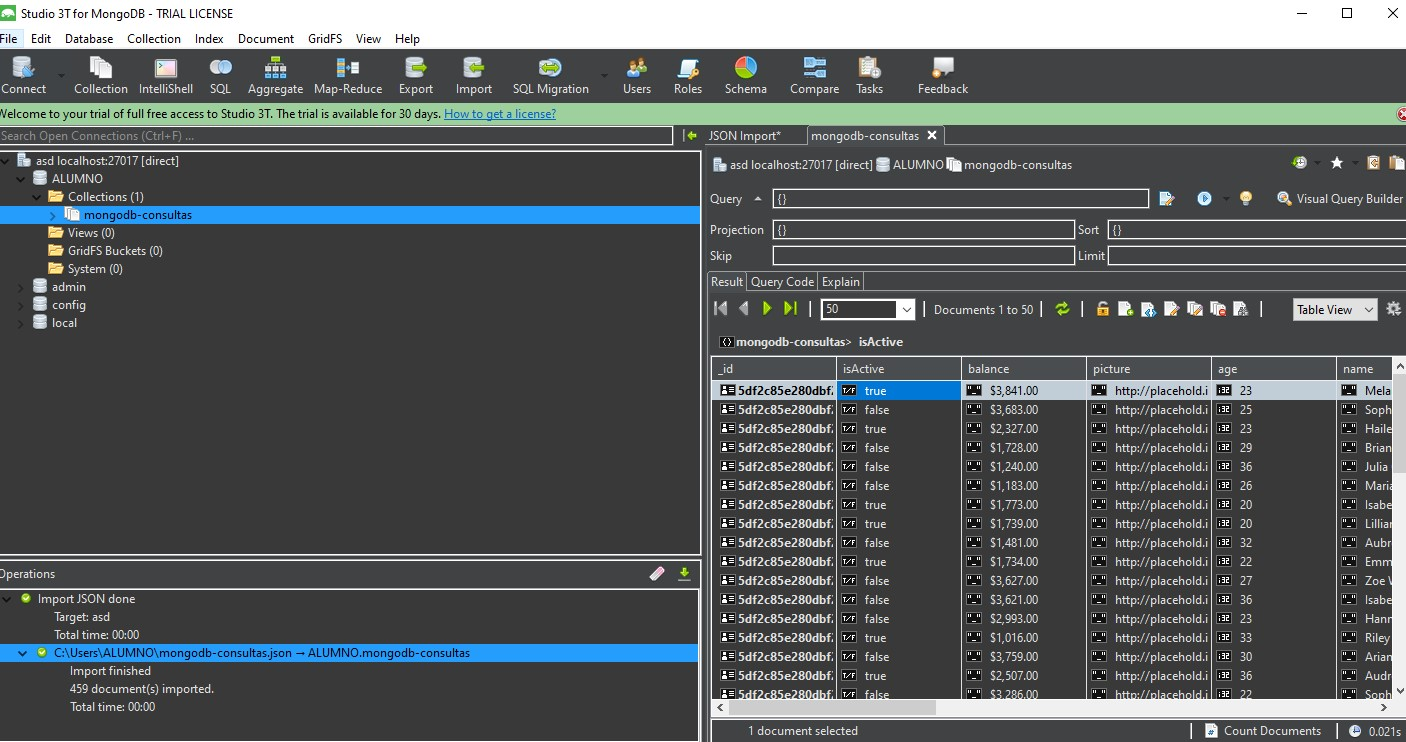
\includegraphics[width=12cm]{./IMAGENES/4} 
	\end{center}
\end{figure}
\subsubsection{\textbf{Mostrando las bases de datos con el comando: show dbs}}
\begin{figure}[H]
	\begin{center}
		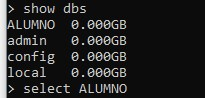
\includegraphics[width=12cm]{./IMAGENES/5} 
	\end{center}
\end{figure}
\subsubsection{\textbf{Mostrando las colecciones de una base de datos con el comando: show collections}}
\begin{figure}[H]
	\begin{center}
		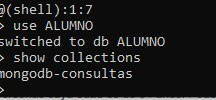
\includegraphics[width=12cm]{./IMAGENES/6} 
	\end{center}
\end{figure}
\subsubsection{\textbf{Mostrando los datos de la coleccion}}
\begin{figure}[H]
	\begin{center}
		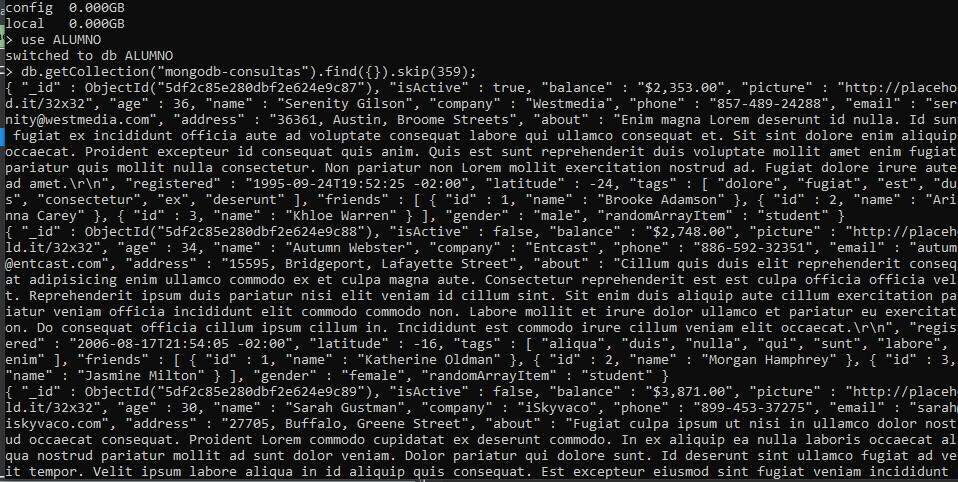
\includegraphics[width=12cm]{./IMAGENES/7} 
	\end{center}
\end{figure}
\subsubsection{\textbf{Mostrando los datos de la coleccion con "PRETTY"}}
\begin{figure}[H]
	\begin{center}
		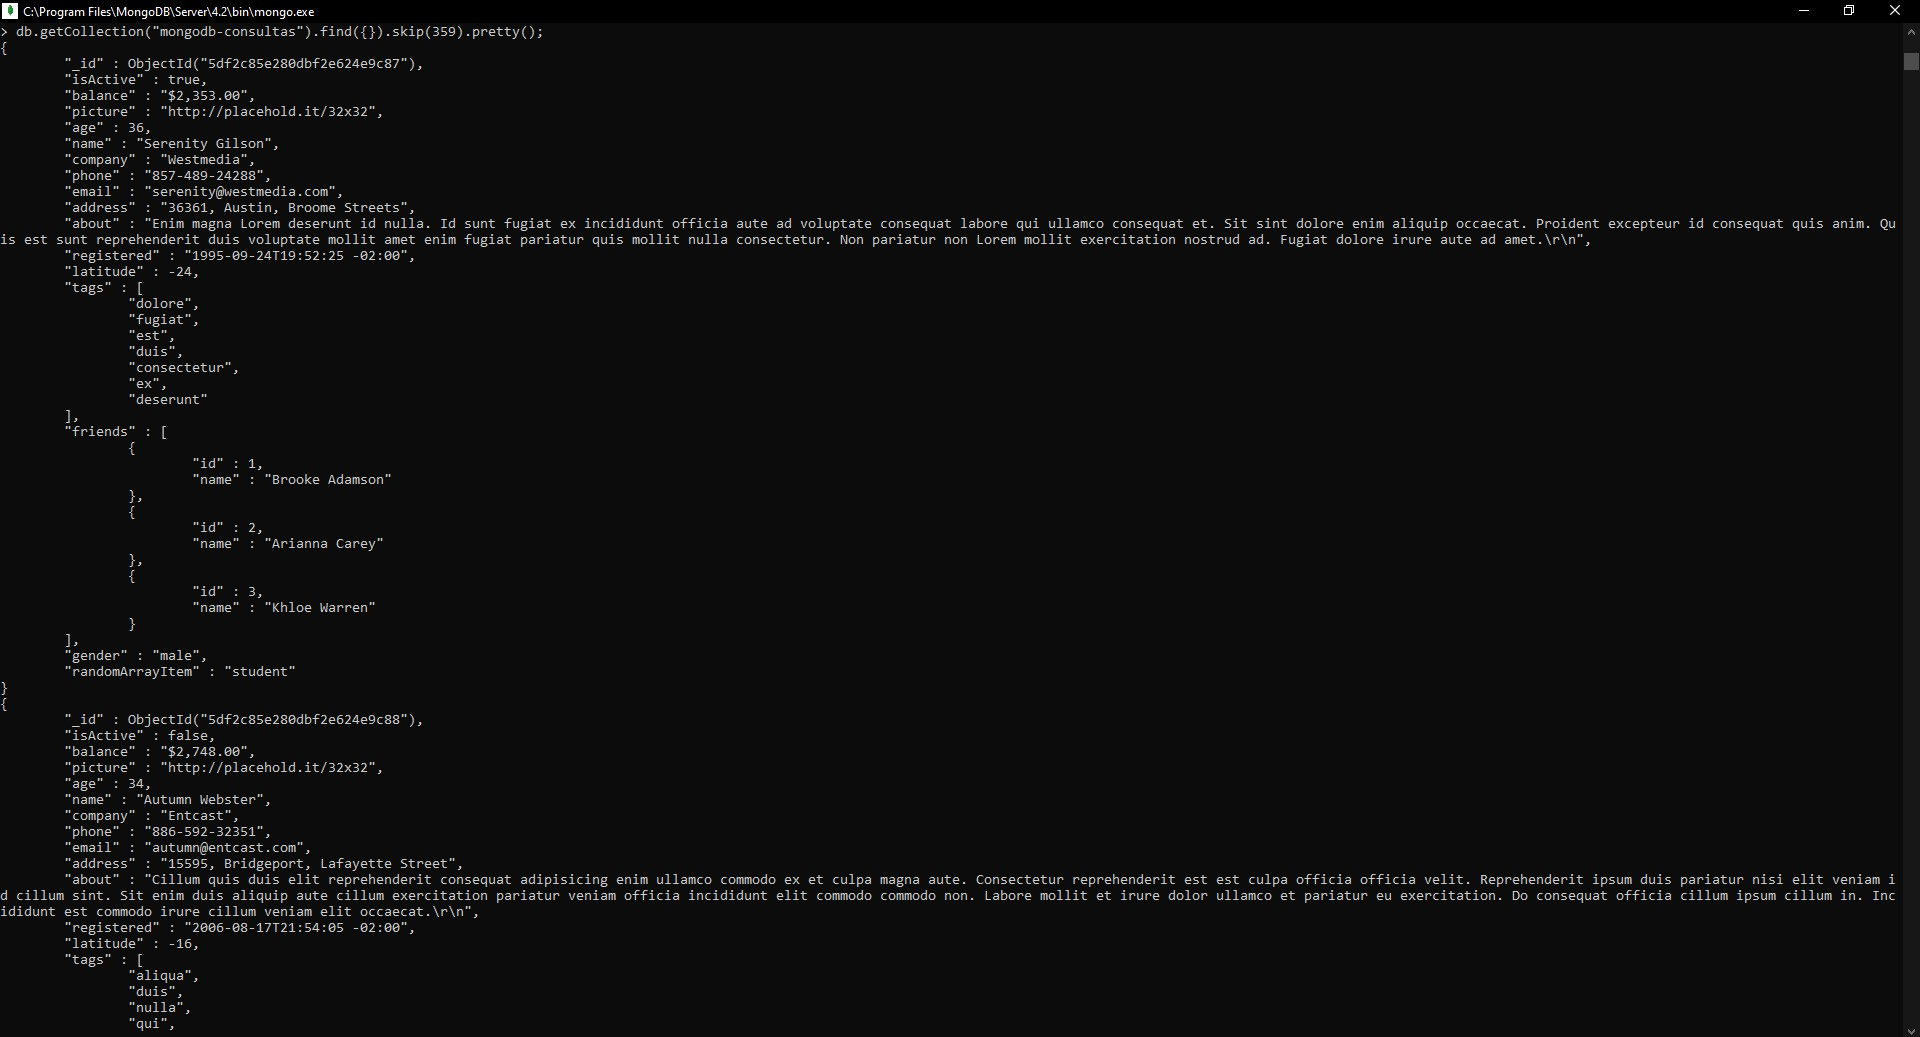
\includegraphics[width=12cm]{./IMAGENES/8} 
	\end{center}
\end{figure}

\subsubsection{\textbf{Paso 3: Explicacion del query en studio 3T}}
\begin{figure}[H]
	\begin{center}
		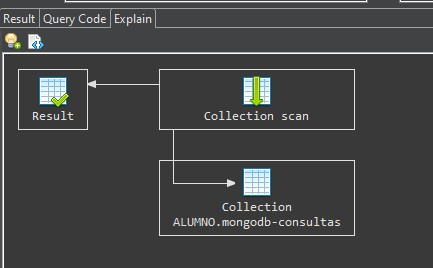
\includegraphics[width=12cm]{./IMAGENES/9} 
	\end{center}
\end{figure}

\begin{figure}[H]
	\begin{center}
		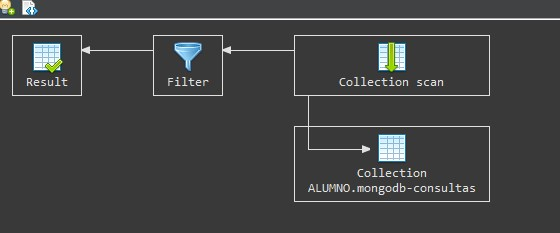
\includegraphics[width=12cm]{./IMAGENES/10} 
	\end{center}
\end{figure}
\subsubsection{\textbf{Paso 4: Querys de busqueda en mongo}}
\begin{figure}[H]
	\begin{center}
		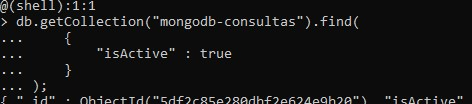
\includegraphics[width=12cm]{./IMAGENES/11} 
	\end{center}
\end{figure}

\begin{figure}[H]
	\begin{center}
		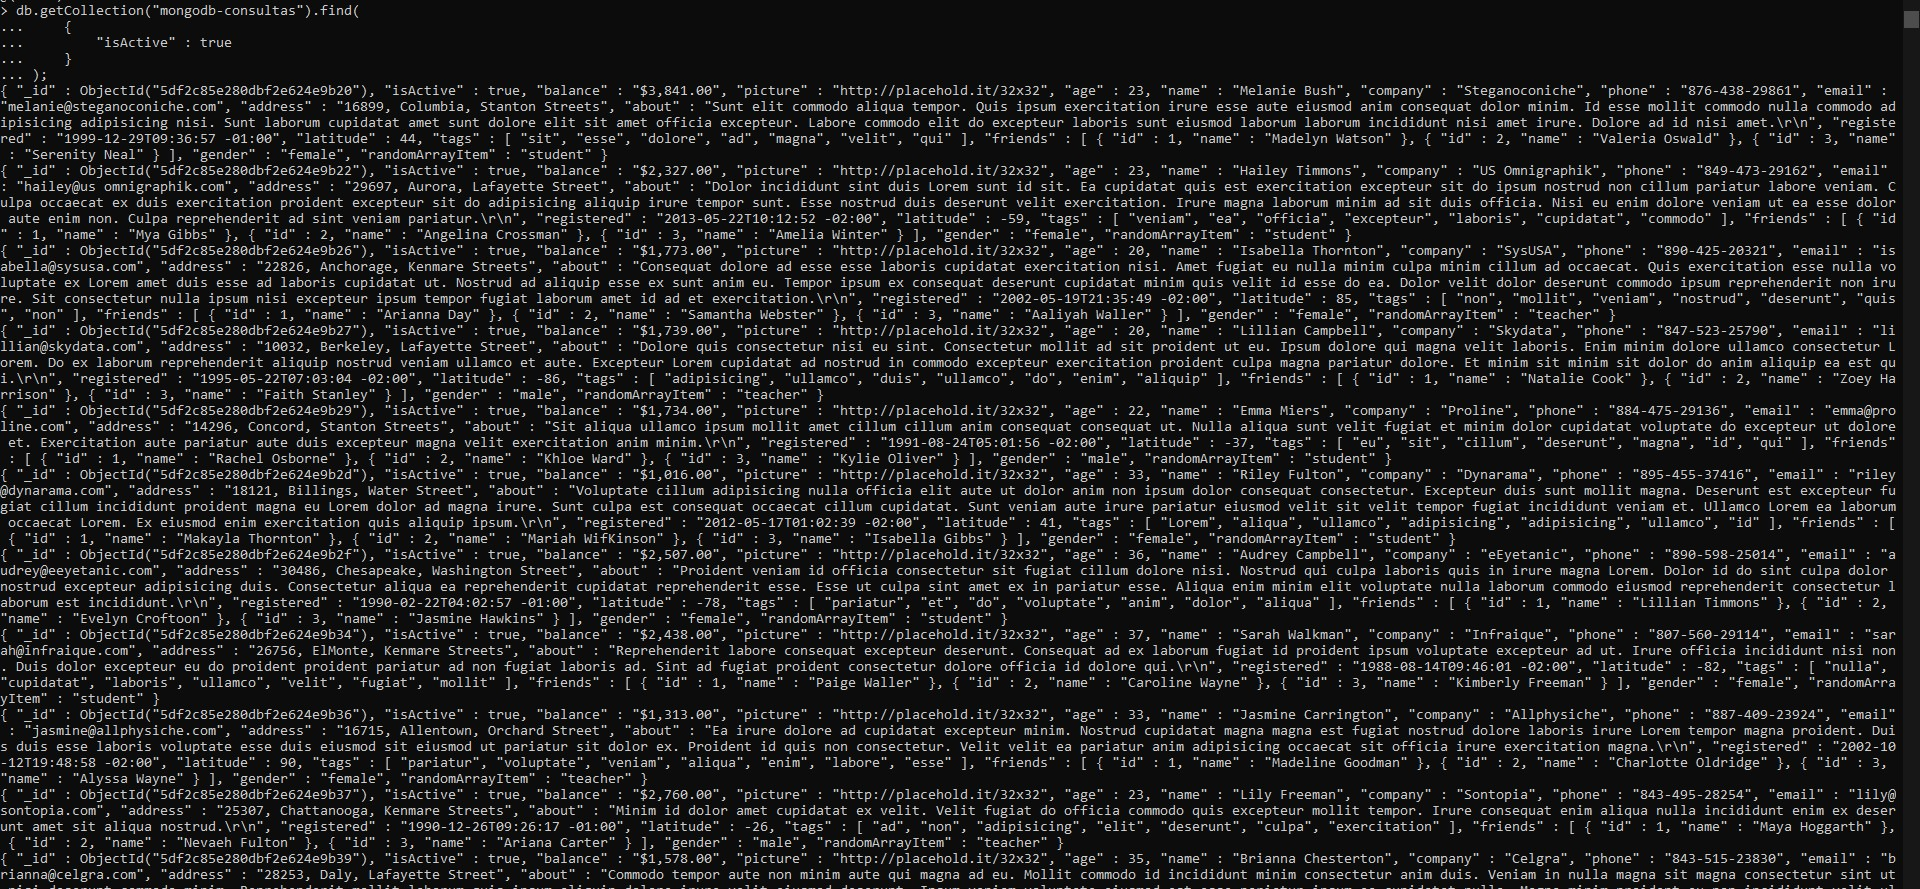
\includegraphics[width=12cm]{./IMAGENES/12} 
	\end{center}
\end{figure}


\section{ANALISIS E INTERPRETACION DE RESULTADOS }
\begin{itemize}
	\item ¿Qué indican los resultados? \\
	Pudimos realizar exitosamente la conexión con mongodb
	\item ¿Que se ha encontrado?\\
	Se ha encontrado una forma rapida y eficiente de trabajar con bases de datos nosql.
\end{itemize}



\section{CONCLUSION}
Mongodb es una base de datos nosql muy flexible y bastante facil de usar, eficiente y con buen rendimiento. Ademas de otorgar un aprendizaje rapido.

\end{document}
